
\documentclass[a4paper,11pt]{article}

\usepackage{amsmath,amssymb,amsfonts,amsthm}    % Typical maths resource packages
\usepackage{graphicx}                           % Packages to allow inclusion of graphics
\usepackage{hyperref}                           % For creating hyperlinks in cross references
\usepackage[authoryear]{natbib}                 % literature reference style
\usepackage[bf]{caption2}
\usepackage[utf8]{inputenc}
\usepackage{tcolorbox}


\usepackage{listings}

% Default fixed font does not support bold face
\DeclareFixedFont{\ttb}{T1}{txtt}{bx}{n}{10} % for bold
\DeclareFixedFont{\ttm}{T1}{txtt}{m}{n}{10}  % for normal

% Custom colors
\usepackage{color}
\definecolor{deepblue}{rgb}{0,0,0.5}
\definecolor{deepred}{rgb}{0.6,0,0}
\definecolor{mypurple}{rgb}{0.627,0.126,0.941}
\definecolor{mygreen}{rgb}{0, 0.5, 0}
\definecolor{lemonchiffon}{rgb}{1, 0.98, 0.8}

% Python style for highlighting
\newcommand\pythonstyle{\lstset{
numbers=left,
backgroundcolor=\color{lemonchiffon},
commentstyle=\itshape\fontsize{9}{1}\color{mygreen},
language=Python,
lineskip={-1.5pt},
basicstyle=\ttm,
otherkeywords={self},             % Add keywords here
keywordstyle=\ttb\color{deepblue},
emph={MyClass,__init__},          % Custom highlighting
emphstyle=\ttb\color{deepred},    % Custom highlighting style
stringstyle=\color{mypurple},
frame=l,                         % Any extra options here
showstringspaces=false            % 
}}

% Python environment
\lstnewenvironment{python}[1][]
{
\pythonstyle
\lstset{#1}
}
{}

% Python for external files
\newcommand\pythonexternal[2][]{{
\pythonstyle
\lstinputlisting[#1]{#2}}}

% Python for inline
\newcommand\pythoninline[1]{{\pythonstyle\lstinline!#1!}}



% -------------------------------
% --- some layout definitions ---
% -------------------------------

% define topline
\usepackage[automark]{scrpage2}
\pagestyle{scrheadings}
\automark{section}
\clearscrheadings
\ohead{\headmark}

% define citation style
\bibliographystyle{ecta}

% define page size, margin size
\setlength{\headheight}{1.1\baselineskip}
\voffset=-2cm
\hoffset=-3cm
\textheight24cm
\textwidth15.5cm
\topmargin1cm
\oddsidemargin3cm
\evensidemargin3cm

% define line line spacing = 1.5
\renewcommand{\baselinestretch}{1.5}

% define second level for `itemizing'
\renewcommand{\labelitemii}{-}




% --------------------------------------
% --------------------------------------
% --------------------------------------
% --- the structure the tex document ---
% ---  (this our recommendation) -------
% frontmatter:
%   - titlepage (mandatory),
%   - acknowledgement,
%   - abstract,
%   - table of contents (mandatory),
%   - list of abbreviations (not mandatory),
%   - list of figures (not mandatory),
%   - list of tables  (not mandatory) .
%
% body of the thesis (the structure of the thesis body is not mandatory, but the list of literature is mandatory):
%   - introduction,
%   - methods,
%   - data,
%   - results,
%   - conclusion,
%   - literature (mandatory),
%   - appendix (figures, tables).
%
% last page:
%   - declaration of authorship (mandatory).
% --------------------------------------
% --------------------------------------
% --------------------------------------

\begin{document}

% -------------------------------
% --- frontmatter: Title page ---
% -------------------------------

\begin{center}

	\begin{center}
      
\includegraphics[scale=0.2,angle=0]{Beuth.png}\\\vspace{2.5cm}
    \end{center}
    
 	{\bf {\huge Python und IoT: MQTT}}\\
    {\normalsize vorgelegt von}\\
    {\bf Thee Vanichangkul \\
    814517} \\\vspace{2cm}

    {\normalsize{\bf Studiengang: Technische Informatik}} \\\vspace{0.5cm}
	{\normalsize Modul: Advanced Python\\\vspace{0.5cm}
	betreut durch: {\bf Prof. Dr. rer. nat. Rüdiger Weis} \\\vspace{8.5cm}
    Berlin, 19.Januar 2017}

\end{center}




% -----------------------------
% --- frontmatter: Contents ---
% -----------------------------
\newpage
\tableofcontents
\ohead[]{Inhaltsverzeichnis}
\clearpage


% ----------------------------------------------------
% --- frontmatter: List of Figures (not mandatory) ---
% ----------------------------------------------------
\newpage
\addcontentsline{toc}{section}{Abkürzungsverzeichnis}

\section*{Abkürzungsverzeichnis}

\begin{tabular}{rp{0.2cm}lp{1cm}rp{0.2cm}l}
    IoT     & &  Internet of Things   & & M2M    & &  Machine to Machine  \\
    TCP     & &  Transmission Control Protocol & & WWW     & &  World Wide Web \\
	URL     & &  Uniform Resource Locator   \\

	
\end{tabular}






% -------------------------------
% --- main body of the thesis ---
% -------------------------------
\newpage
\pagestyle{plain}
\setcounter{page}{1}    % start page numbering anew
\pagenumbering{arabic}  % page numbers in arabic style


\section{Motivation}
Als ich noch bei Wincor Nixdorf als Werkstudent gearbeitet habe, habe ich viele Testskripte für Kassensysteme in Ruby geschrieben. Meine Interesse an Skriptsprachen hat sich seitdem stark intensiviert. Danach habe ich auch als Werkstudent bei Siemens angefangen Skripte in Python zu Schreiben und habe gleichzeitig auch mehr über IoT gelesen.Obwohl Ich die Syntax von Ruby schöner als Python finde, ist Python mehr populär und hat mehr Bibliotheken bezüglich Iot. Deswegen habe ich in meiner Freizeit Python und Iot ausprobiert. Im Rahmen des Moduls Advanced Python wurde mir die Möglichkeit geboten mich in ein für mich interessantes Python Thema zuvertiefen.

\section{Was ist IoT?}
Internet of Things (IoT) bzw. Das Internet der Dinge ist die Digitalisierung von physischen Objekten, die normallerwise in der "Offline-welt" leben wie Toaster und Kühlschränke und deren Vernetzung über das Internet. Um die Dinge (Geräte) im Netz zu vernetzen braucht man aber ein 
Kommunikationsprotokoll, die geeingnet ist um den Anforderungen des Internet of Things zu erfüllen. Mein ausgewältes Protokoll ist MQTT.

\section{Was ist MQTT?}

\includegraphics[scale=0.4]{mqtt.png}

Das Protokoll MQTT wurde 1999 von Andy Stanford-Clark (IBM) und Arlen Nipper (Cirrus Link) als ein M2M-Kommunikationsprotokoll für SCADA-Systeme zum Monitoring von Ölpipelines entwickelt.
Es ist ein auf TCP basierendes, leichtgewichtiges und schlankes  Protokoll.
Es bietet bandbreit- und powerlimitierenden Geräten eine Möglichkeit, miteinander zu kommunizieren. Das Protokoll MQTT ist auch clientseitig sehr einfach zu implementieren.
Das Protokoll ermöglicht eine effiziente Datenübertragung und sichere Zustellung der Daten in instabiles Netz. Da die Zahlen der "Smart-Geräte" stark zugestiegen ist und diese Anforderungen heute immer noch aktuell sind wurde der Source Code 2010 unter einer freien Lizenz veröffentlicht. Heute ist MQTT eines der besten und meist benutzen IoT Protokoll.

\section{Warum MQTT?}
Es stellt sich die Frage, welches Kommunikationsprotokoll geeignet ist um den Anforderungen des Internet of Things gerecht zu werden. Neben dem Klassiker unter den Internetprotokolle in, HTTP, etabliert sich das Protokoll MQTT immer mehr zu einem IoT-Standard. Das sehr schlanke und leichtgewichtige Kommunikationsprotokoll punktet durch folgende Eigenschaften:

\begin{itemize}
\item MQTT ist schlank und leichtgewichtig und sehr einfach zu implementieren.
\item MQTT implementiert das Publish / Subscribe Pattern und erlaubt damit echtes Push-Messaging zwischen allen Kommunikationsteilnehmern.
\item MQTT gewährleistet durch verschiedene Quality of Service Levels die Datenübertragung in instabilen Netzen, wie etwa Mobilfunknetzen.
\item MQTT besitzt einen minimalen Protokolloverhead.
\item MQTT ist Session-Aware. Das bedeutet, Metainformationen müssen im Idealfall nur einmal übertragen werden, da der Server die Daten nach einem Verbindungsabbruch weiterhin vorhält.
\item MQTT ist datenagnostisch. Es ist daher möglich, Daten in jedem möglichen Format zu übertragen.
\end{itemize}


All diese Eigenschaften machen MQTT zu einer sehr guten Wahl, da mittels dem Publish / Subscribe Pattern eine hohe Skalierbarkeit erreicht werden kann und mit dem minimalen Overhead und verschiedenen Quality of Service Levels können selbst instabile und teure Kommunikationskanäle wie Mobilfunknetze und Satellitenübertragung kosteneffizient genutzt werden.
\footnote{https://www.informatik-aktuell.de/betrieb/netzwerke/internet-der-dinge-protokolle-verfahren-und-integration-von-mqtt.html}

\pagebreak
\section{Wie Funktioniert MQTT?}

\subsection{Publish/Subscribe}
\begin{center}
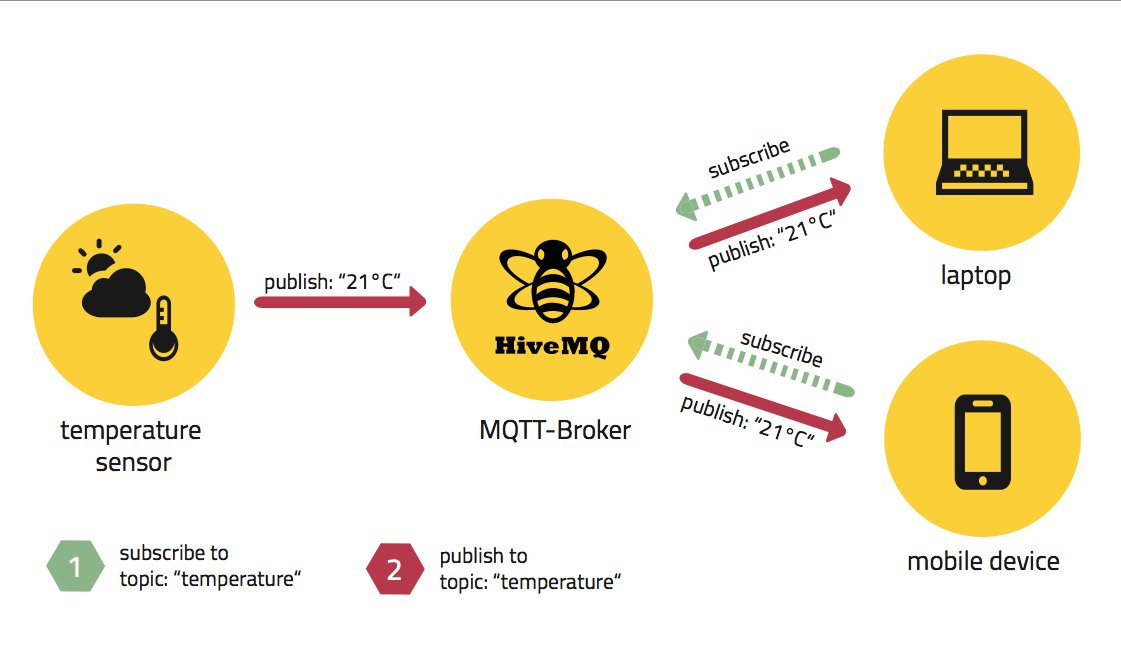
\includegraphics[scale=0.4]{hivemq.png}
src: Dominik Obermaier http://www.hivemq.com/
\end{center}
MQTT benutzt das Publish/subscribe das heißt Jeder MQTT-Client, der Nachrichten für dieses Topic empfangen möchte, abonniert es beim Message Broker.
Da die interessierten Clients beim Eintreffen neuer Nachrichten durch den Broker benachrichtigt werden, anstatt selbst beim Server nach Änderungen zu fragen, wird eine hocheffiziente Kommunikation zwischen den Teilnehmern gewährleistet.
Somit ist eine echte Push-Kommunikation möglich. Entscheidend ist, dass die Teilnehmer der Kommunikation nichts voneinander wissen, da jeder Client nur den Message Broker kennt, nicht jedoch die anderen Teilnehmer.
\footnote{https://jaxenter.de/iot-allrounder-27208}
	
\subsection{Topic}
\begin{center}
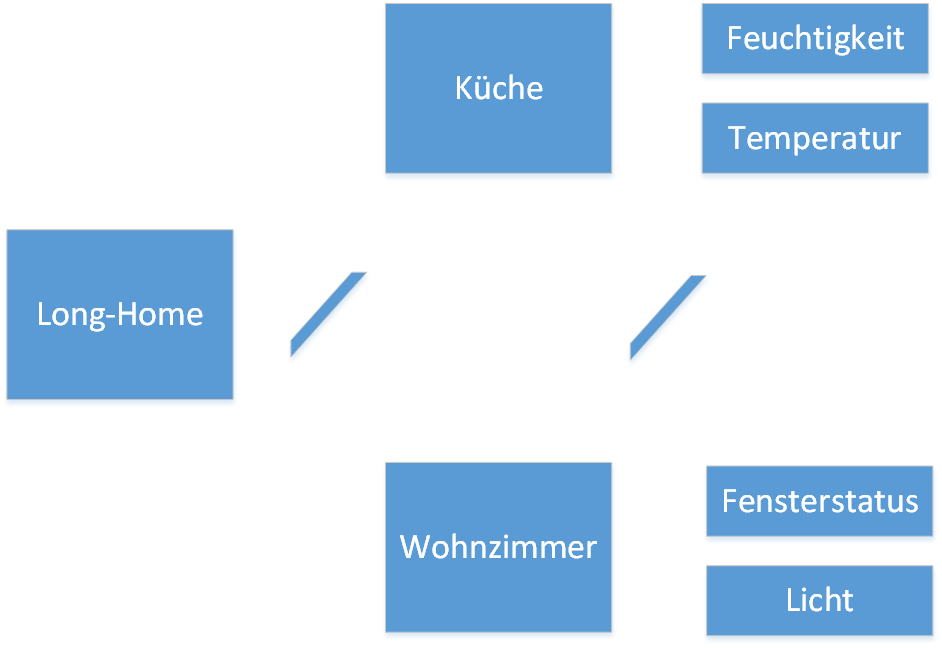
\includegraphics[scale=0.6]{mqtttopic.png}
\end{center}
Topics sind einfache Zeichenketten welche eine Art Nachrichten-Hierarchie abbilden und mit einer einfachen URL vergleichbar sind. Hier sind paar wichtige Beispiele wie man mit Topics in MQTT benützen kann.

\begin{tcolorbox}[colback=green!5,colframe=green!40!black,title=Nur die Temperatur aus Longs Küche]
Subscriber: Long-Home/Küche/Temperatur
\end{tcolorbox}

\begin{tcolorbox}[colback=green!5,colframe=green!40!black,title=Alles aus Longs Wohnzimmer]
Subscriber: Long-Home/Wohnzimmer/\#
\end{tcolorbox}

\begin{tcolorbox}[colback=green!5,colframe=green!40!black,title=Alles aus Long-Home]
Subscriber: Long-Home/\#
\end{tcolorbox}

\begin{tcolorbox}[colback=green!5,colframe=green!40!black,title=Temperatursensor wert publishen]
Publisher: Long-Home/Küche/Temperatur + "wert"
\end{tcolorbox}


\pagebreak
\subsection{Quality of service (QoS)}
Da MQTT auf dem TCP Protokoll basiert, kommt es von Haus aus mit einer großen Zuverlässigkeit in Sachen Datenaustausch. Allerdings kann es gerade im mobilen Bereich, zu Verbindungsengpässen oder gar Ausfällen kommen. Zu diesem Zweck wurde das Protokoll um den Quality of Service Mechanismus erweitert, welcher das Übertragen von Nachrichten garantiert. Dabei unterscheidet MQTT in drei Servicequalitäten:
\begin{itemize}
\item QoS = 0: fire and forget
\item QoS = 1: Nachricht kommt mindestens einmal an
\item QoS = 2: Nachricht kommt genau einmal an
\end{itemize}

Je nach Einsatzgebiet oder Gewichtung der zu versendeten Nachricht, kann der MQTT-Client selbst entscheiden welcher QoS für ihn am geeignetsten ist. Um bei unserem Beispiel mit den Flotten-Fahrzeugen zu bleiben: Nehmen wir an, das Fahrzeug sendet im Sekunden-Takt seine Position an den Broker. Hier wäre es angebracht die Nachricht mit einem Wert von 0 zu versenden, da eine einzelne verloren gegangene Geo-Position verkraftbar ist (da in einer Sekunde bereits die nächste folgt) und dadurch nicht unnötiger Rückkopplungs-Overhead entsteht. Die Servicequalität von 2 wird beim subscriben eines Clients am Broker eingesetzt. Hier ist es wichtig, dass die Abonierung nur ein einziges mal ankommt und der Client sich nicht versehentlich doppelt registiert, wenn z. B. die Rückantwort des Servers verloren ging.
\footnote{http://www.sic-software.com/das-mqtt-protokoll-1/}

\subsection{Last Will Testament (LWT)}

MQTT Clients können beim Verbinden mit dem MQTT Broker eine Nachricht als sog. "Last Will and Testament" angeben. Falls nun der Client unerwartet die Verbindung zum MQTT Broker verliert, sendet der Broker diese Nachricht an alle Subscriber. Damit ist es möglich, interessierte Clients mit einer Nachricht zu informieren, dass ein anderer Client nicht mehr online ist. Sehr häufig wird dieser Mechanismus verwendet um schnell auf Probleme einzelner Clients reagieren zu können, da man sofort ein Feedback bekommt, falls es Störungen gibt.

\begin{python}
client = mqtt.Client(client_id="1234")

# so konfigurioert man LWT
client.will_set(topic, payload="Unexpected disconnect", qos=0,
retain=False)
client.connect("broker.mqttdashboard.com", 1883, 60)

# do work

client.disconnect()
\end{python}

\section{Python und MQTT}
Eclipse Paho ist ein Projekt unter dem Schirm der Eclipse Foundation, das MQTT-Clientimplementierungen in verschiedenen Programmiersprachen zur Verfügung stellt. Das sind neben C die folgenden: C++, C\#, Python, JavaScript, Go und natürlich auch Java. Das Paho-Projekt existiert seit 2012, die Java- und C-Implementierungen werden jedoch seit vielen Jahren bei IBM, die auch die initiale Implementierungen bereitgestellt haben, eingesetzt. Sie sind für den produktiven Einsatz freigegeben. Neben einem synchronen API bietet Paho auch ein asynchrones API, das mehr Performance verspricht, dafür etwas komplizierter in der Benutzung ist. In den folgenden Beispielen wird das synchrone Paho API verwendet.

\subsection{So installiert man MQTT für Python}
paho-mqtt ist kompatibel mit Python 2.7 und 3.X und kann man ganz einfach installieren von Terminal oder Konsole mit dem foldenden Befehl.

\begin{tcolorbox}[colback=green!5,colframe=green!40!black,title=Installation]
\$ pip install paho-mqtt
\end{tcolorbox}
	
\subsection{Test Programme}
Zum testen habe ich 2 MQTT Broken benütz. Bei Mqttdashboard.com kann man MQTT Applikationen kosten frei testen. Und der 2. Broker habe ich Lokal auf mein Raspberry Pi 3 installiert.

\pagebreak

Subscribe:

In diesem Beispiel Abonniere ich das Topic "testtopic/thee" und gebe ich alle kommende Nachrichte auf dem Bildschrim

\begin{python}
import paho.mqtt.client as mqtt

def on_connect(client, userdata, rc):
    print("Connected with result code "+str(rc))
    client.subscribe("testtopic/thee")

#Beim erhalten einer Nachricht, gibt das Programm das gesammte-
#Payload auf der Konsole

def on_message(client, userdata, msg):
    print(str(msg.payload))

client = mqtt.Client(client_id="1234")
client.on_connect = on_connect
client.on_message = on_message

client.connect("broker.mqttdashboard.com", 1883, 60)

client.loop_forever()
\end{python}

Publish:

Hier publiziere ich zufällige temperatur Werte mit einem intervall von 5 Sekunden an "test/topic"

\begin{python}
import time
import random

import paho.mqtt.client as mqtt

def on_connect(client, userdata, flags, rc):
    print("Connected with result code " + str(rc))

client = mqtt.Client()
client.on_connect = on_connect

client.connect("localhost", 1883, 60)

client.loop_start()

while True:
    time.sleep(5)
    temp = random.randrange(-20, 40, 3)
    client.publish("test/topic", "Temperature = %d" % temp)
\end{python}

\pagebreak
\section{Quellen}
\begin{itemize}
\item http://mqtt.org/
\item https://pypi.python.org/pypi/paho-mqtt/1.2
\item https://www.dinotools.de/2015/04/11/mosquitto-als-mqtt-broker/
\item https://www.dinotools.de/2015/04/12/mqtt-mit-python-nutzen/
\item https://www.informatik-aktuell.de/betrieb/netzwerke/internet-der-dinge-protokolle-verfahren-und-integration-von-mqtt.html
\item http://www.sic-software.com/das-mqtt-protokoll-1/
\end{itemize}
	


%\input{methods}
\newpage
%\input{data}
\newpage
%\input{results}
%\input{conc}



% ----------------
% --- appendix ---
% ----------------
\appendix

% literature
\newpage
\addcontentsline{toc}{section}{References}
%\bibliography{literature}

% figures (not mandatory)
\newpage
%\input{app_figures}

% tables (not mandatory)
\newpage
%\input{app_tables}



% --------------------------------------------
% --- last page: Declaration of Authorship ---
% --------------------------------------------

\newpage
\thispagestyle{empty}
%\input{authorship}


\end{document}
